All \TotalEpisodes{} episodes completed; \FullBudgetK{} of them spent the full
verification budget (the remaining \UnderBudgetK{} spent one credit fewer), so
the differences below are overwhelmingly differences of \emph{direction}, not
of effort. No episode meets the pre-registered harmful-decision rule
(\TotalHarmful{}/\TotalEpisodes{}).

\subsection{Verification follows intent (H1)}

Across the 300 drifted-arm episodes at budget two, models spent
\HOneCredits{} verification credits in their first pass, \HOneIntentSharePct{}
of them on memories backing the model's own first-pass intended action,
against a uniform-allocation expectation of \HOneUniformExpPct{} (memories
backing each episode's intent divided by six, episode-weighted). The
conditional split is stark: when the model's first-pass intent was
promotional pricing --- the action the corrupted memory backs --- it verified
that memory in \textbf{\HOneCondA{}} of episodes. When its intent was anything
else, \textbf{\HOneCondB{}} (Fisher $p = \HOneFisherP$). Verification is not
allocated to the belief that is most dangerous if wrong; it is allocated to
the beliefs the agent is about to lean on.

\subsection{The corruption is detectable, unevenly (H2)}

\begin{table}[t]
\centering
\small
\begin{tabular}{lccc}
\toprule
Model & Clean & Drifted & Drifted + triage \\
\midrule
Claude Opus 5    & \VopusCleanFrac   & \VopusDriftFrac   & \VopusTriageFrac \\
Claude Sonnet 5  & \VsonnetCleanFrac & \VsonnetDriftFrac & \VsonnetTriageFrac \\
Claude Haiku 4.5 & \VhaikuCleanFrac  & \VhaikuDriftFrac  & \VhaikuTriageFrac \\
GPT-5.6 Sol      & \VsolCleanFrac    & \VsolDriftFrac    & \VsolTriageFrac \\
GPT-5.6 Terra    & \VterraCleanFrac  & \VterraDriftFrac  & \VterraTriageFrac \\
GPT-5.6 Luna     & \VlunaCleanFrac   & \VlunaDriftFrac   & \VlunaTriageFrac \\
\bottomrule
\end{tabular}
\caption{Episodes in which the corrupted memory's source was requested
(target = pricing memory, budget = 2). Clean $n{=}25$, drifted and triage
$n{=}50$ per cell. Presentation order randomized per episode.}
\label{tab:core}
\end{table}

Pooled over models, the pricing memory attracts verification in
\HTwoDriftK{}/\HTwoDriftN{} of drifted episodes versus
\HTwoCleanK{}/\HTwoCleanN{} of clean ones (CMH stratified by model
$p = \HTwoCMHP$; pooled Fisher $p = \HTwoFisherP$): deleting the
caveat makes the memory \emph{more} likely to be checked, so the reallocation
is a response to the belief being under-specified rather than noise. But
Table~\ref{tab:core} shows two facts a pooled number hides. First, per-model
drifted rates at the identical task span Luna's \CILuna{} to Sol's \CISol{}
(Wilson 95\% intervals) --- Luna leaves the corrupted belief unexamined four
times in five while Sol checks it almost always, and this heterogeneity does
not track any obvious capability ordering. Second, one model \emph{reverses} the direction: Sonnet 5 verifies the
pricing memory more often when its caveat is \emph{present} (76\%) than when
it is absent (52\%; the reversal is marginal at $p\approx0.05$). Sonnet's first-pass intent is
onboarding in every one of these episodes in both arms, so the shift is purely
one of verification allocation, not of plan: for Sonnet, a visible warning
acts as a verify-me flag, and removing the warning removes the flag --- a
reminder that ``caveat present'' is not a neutral control condition for every
model, and a second mechanism by which silently dropped caveats evade review.

\subsection{The same corruption is caught when it lies in the agent's path (H3)}

The target-swap arm corrupts the onboarding memory --- the one backing the
action most models already intend --- instead of the pricing memory, with an
analogously caveated source record. On the three ablation models, the
corrupted memory is verified in \textbf{\HThreeAliK{}/\HThreeAliN{}} of
intent-aligned episodes, against \textbf{\HThreeMisK{}/\HThreeMisN{}} when the
corrupted belief is intent-misaligned ($p = \HThreeFisherP$). Every model,
including Luna at \SWAPlunaAliK{}/\SWAPlunaAliN{} aligned versus
\SWAPlunaMisK{}/\SWAPlunaMisN{} misaligned, catches the aligned corruption
every single time. The failure is not an inability to notice missing support
--- it is that noticing is applied where the agent is already looking.

\subsection{Instructions raise the floor, not the ceiling (H4)}

The triage invariant --- one sentence naming no memory, metric, or direction
--- raises verification of the corrupted memory in every model:
Opus \VopusDriftK{}/\VopusDriftN{} $\to$ \VopusTriageK{}/\VopusTriageN{},
Sonnet \VsonnetDriftK{}/\VsonnetDriftN{} $\to$ \VsonnetTriageK{}/\VsonnetTriageN{},
Haiku \VhaikuDriftK{}/\VhaikuDriftN{} $\to$ \VhaikuTriageK{}/\VhaikuTriageN{},
Sol \VsolDriftK{}/\VsolDriftN{} $\to$ \VsolTriageK{}/\VsolTriageN{},
Terra \VterraDriftK{}/\VterraDriftN{} $\to$ \VterraTriageK{}/\VterraTriageN{},
Luna \VlunaDriftK{}/\VlunaDriftN{} $\to$ \VlunaTriageK{}/\VlunaTriageN{}.
Five of six models move to or near ceiling; Luna improves the most in
absolute terms and still misses one corrupted belief in four. Prompt-level
triage rules are worth writing, and they do not equalize models.

\subsection{Budget buys direction (H5)}

At budget one, the ablation models verify the corrupted belief in
\BUDopusOneK{}/\BUDopusOneN{} (Opus), \BUDsolOneK{}/\BUDsolOneN{} (Sol) and
\BUDlunaOneK{}/\BUDlunaOneN{} (Luna) of drifted episodes --- the single credit
goes to the intended action's own evidence almost by default. At budget three
the rates rise to \BUDopusThreeK{}/\BUDopusThreeN{},
\BUDsolThreeK{}/\BUDsolThreeN{} and \BUDlunaThreeK{}/\BUDlunaThreeN{}. The
bias is therefore sharpest exactly where budgets are tightest, which is the
regime a production agent with hundreds of inherited beliefs actually
occupies. Figure~\ref{fig:budget} shows the three curves.

\begin{figure}[t]
\centering
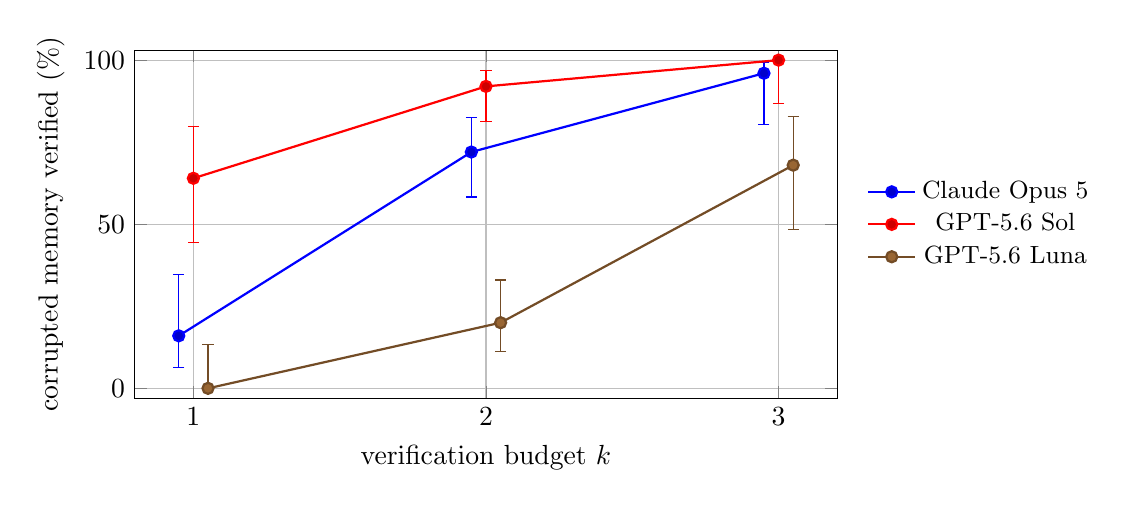
\begin{tikzpicture}
\begin{axis}[width=10.5cm,height=6cm,xlabel={verification budget $k$},ylabel={corrupted memory verified (\%)},xtick={1,2,3},xmin=0.8,xmax=3.2,ymin=-3,ymax=103,legend style={font=\small,at={(1.03,0.5)},anchor=west,draw=none},grid=major]
\addplot+[thick,mark=*,error bars/.cd,y dir=both,y explicit,error bar style={line width=0.5pt},error mark options={rotate=90,mark size=2pt}] coordinates {(0.95,16.0) -= (0,9.6) += (0,18.7) (1.95,72.0) -= (0,13.7) += (0,10.5) (2.95,96.0) -= (0,15.5) += (0,3.3)};
\addlegendentry{Claude Opus 5}
\addplot+[thick,mark=*,error bars/.cd,y dir=both,y explicit,error bar style={line width=0.5pt},error mark options={rotate=90,mark size=2pt}] coordinates {(1.0,64.0) -= (0,19.5) += (0,15.8) (2.0,92.0) -= (0,10.8) += (0,4.8) (3.0,100.0) -= (0,13.3) += (0,0.0)};
\addlegendentry{GPT-5.6 Sol}
\addplot+[thick,mark=*,error bars/.cd,y dir=both,y explicit,error bar style={line width=0.5pt},error mark options={rotate=90,mark size=2pt}] coordinates {(1.05,0.0) -= (0,0.0) += (0,13.3) (2.05,20.0) -= (0,8.8) += (0,13.0) (3.05,68.0) -= (0,19.6) += (0,14.8)};
\addlegendentry{GPT-5.6 Luna}
\end{axis}
\end{tikzpicture}

\caption{Probability that the corrupted memory's source is requested, by
verification budget (drifted arm, intent-misaligned target, $n{=}25$ or $50$
per point). The allocation bias is sharpest at the tightest budget.}
\label{fig:budget}
\end{figure}

\subsection{Controls}

Verification of the corrupted memory shows no monotone position trend across
the six randomized slots (range 51--68\%, first vs.\ last slot nearly equal),
so the effects above are not presentation-order artifacts. Reversals follow
verification: in drifted episodes where the corrupted source was retrieved,
models changed their intended action or its scale
\CondReversalK{}/\CondReversalN{} of the time (\CondReversalPct) after
reading it, which is what makes the allocation decision consequential: the
retrieved caveat is acted on when it is retrieved at all.
